\documentclass[12pt]{article}

\usepackage[utf8]{inputenc}
\usepackage[brazil]{babel}
\usepackage{graphicx}
\usepackage[table]{xcolor}
\usepackage{tabularx}
\usepackage{hyperref}
\usepackage{booktabs}
\usepackage{bookmark}

\begin{document}
\title{TerraCota\\Game Design Document}
\author{NullPointer Corporation}
\date{v0.9}
\maketitle

\newpage

\begin{table}[h]
  \centering
  \begin{tabular}{ccll}
    \toprule
    \textbf{Versão} & \textbf{Data} & \textbf{Autor} & \textbf{Descrição} \\
    \midrule
    0.1 & 22/04/2015 & Carlos Oliveira  & Versão Inicial \\
    \rowcolor[gray]{0.9}
    0.2 & 20/05/2015 & Álvaro Fernando & Adicionando novas seções \\
    0.3 & 22/05/2015 & Carlos Oliveira & Front-end \\
    \rowcolor[gray]{0.9}
    0.4 & 30/05/2015 & Álvaro Fernando & Objetos Colecionáveis \\
    0.5 & 17/06/2015 & Álvaro Fernando & Telas \\
    \rowcolor[gray]{0.9}
    0.6 & 17/06/2015 & Álvaro Fernando & Câmera e HUD \\
    0.7 & 26/06/2015 & Álvaro Fernando & Personagem principal \\
    \rowcolor[gray]{0.9}
    0.7 & 05/07/2015 & Álvaro Fernando & Power Ups e Sistema de Pontuação \\
    0.8 & 07/07/2015 & Álvaro Fernando & Pricipais Personagens do Mundo \\
    \rowcolor[gray]{0.9}
    0.9 & 07/07/2015 & Álvaro Fernando & Progresso do Jogo \\
    \bottomrule
  \end{tabular}
  \caption{Histórico de Revisões}
\end{table}

\newpage

\tableofcontents

\newpage

\listoffigures

\newpage
\section{Objetivo do jogo}

\subsection{Conceito do jogo}
O jogo terá uma movimentação semelhante a games do estilo beat'em up (briga de
rua em português), como principais referências e exemplos os jogos Little
Fighter 2 (PC), Captain Commando (SNES), Double Dragon (SNES).

A temática será a de um mundo pós-apocalíptico, onde várias tecnologias se
extinguiram e a humanidade volta a comunicar-se de forma arcaica por meio de
figuras e indicações corporais. O jogador terá que, entre outros desafios,
resolver puzzles decifrando códigos audiovisuais para completar as quests.

Todos os membros da equipe estão cientes do conceito do jogo. No diretório
deste arquivo é possível visualizar algumas imagens feitas pelo artista Pedro
Braga que podem auxiliar no entendimento da temática.

\subsection{Principais características}
Uma das características mais interessantes do jogo são o modo como os gêneros
aventura e puzzle interagem entre si, fazendo com o que o jogador precise
pensar e decifrar qual será sua missão, pois as informações serão dadas
através de símbolos.

A movimentação é em dois eixos, vertical e horizontal, mais do que um jogo de
plataforma, que contém só um, desconsiderando a função de pular, também é uma
característica diferenciada do jogo, pois traz um modo de exploração em visão
em múltiplos planos. A inspiração desse estilo de movimentação veio,
principalmente, do jogos Capitão Comando, Little Fighter 2 e Double Dragon.

Não estará presente no jogo elementos relacionados à economia e/ou obtenção de
recursos, tais como dinheiro, moeda, cristais, etc. Levando em consideração o
conceito do jogo, a humanidade se abstém de um sistema monetário, colocando em
prática a barganha para obtenção de itens, peças, alimentos, etc.

Também não estará presente modificadores de estado (ou power ups). O jogo não
conterá um sistema de pontuação, portanto não será contabilizado nenhum tipo
de ponto medidos geralmente por moedas, tempo, barras, etc.

\section{Visão geral}
O jogo é dividido em 5 segmentos, ou 5 capítulos:
\begin{enumerate}
\item Tutorial pra interação com o mundo, tarefas simples como "ir falar com o
carteiro" ou "buscar o leite na despensa" para o jogador se acostumar com a
linguagem do jogo. Este tutorial será exibido na forma de uma cutscene, dessa
forma não haverá interação do usuário.
Após essa pequena introdução é revelado que alguns morcegos/monstros invadiram
o último andar da torre, e o jogador deve ir se livrar deles.

\item O jogador precisa de alguma arma, então deve ir até o ferreiro para
conseguir uma espada simples. Ele sobe até o último andar da torre e elimina os
morcegos, mas por acidente desperta o mecanismo de defesa da torre, que o ataca
(chefão 1).
Durante a batalha, a espada do Inti se prova ineficaz (pode talvez quebrar)
porém ele acha uma espada fincada na parede próxima ao chefão. Ele remove a
espada (o que destranca a porta para a saída pro mundo afora) e usa ela pra
derrotar o chefão.
Ao derrotar o chefão uma porta atrás dele se revela e abre, revelando um mundo
inteiro do lado de fora.

\item Curioso pra explorar o mundo, Inti sobe no "elevador" do lado de fora da
torre e desce para o chão, entrando numa floresta.
Ao caminhar pela floresta ele encontra a Killa, sentada em um galho. Ela percebe
ele, sorri, chama ele e sai andando. A missão se torna seguir a Killa.
Ela guia ele até a aldeia dela, e introduz o pai dela (cacique) e o jogador se
torna livre a explorar os arredores e a realizar sidequests (se der tempo de
desenvolvê-las), a missão se torna retornar à torre e contar para os pais sobre
a existência de mais pessoas além das que vivem na torre com ele.

\item Ele retorna para a torre, Killa fica para trás porque o pai dela não deixa
ela sair da floresta, e tenta convencer as pessoas sobre o mundo de fora. Ninguém
acredita nele nem segue ele quando ele tenta mostrar. Ele decide procurar um
artefato valioso pra provar a existência do mundo lá fora (estamos pensando em
fazer um artefato que seja presente em toda torre, porém só um. Ao trazer um de
outra torre ele prova a existência dela).
Então ele volta para a floresta e Killa se junta a ele mais uma vez, e ajuda ele
a chegar na torre onde ela vivia. Numa região alagada da floresta. Os dois
entram na torre.

\item A torre abandonada, cheia de puzzles. Ao chegar na câmara onde o artefato
está, eles percebem que precisam de uma chave pra destrancar ela. Quando eles
encontram a chave, o chefão a engole antes que eles consigam pegar ela. O objetivo
se torna derrotar o chefão pra pegar a chave de volta, e então conseguir o artefato.
Com o artefato em mãos, o Inti volta pra torre, prova a existência do mundo afora,
e o jogo termina com a população na frente da porta, olhando o mundo do lado de fora
\end{enumerate}

\section{Requisitos Tecnológicos}

\subsection{Ferramentas de codificação}
O jogo Terracota será desenvolvido na linguagem de programação C++, linguagem
esta de uso geral e caracterizada pelo versatilidade e alto desempenho. Bastante
usada no setor de jogos eletrônicos. Para compilação do código será utilizado o
Clang, versão 3.4.Os editores de texto utilizados para a codificação serão o Vim
(open-source) e o Sublime-Text (proprietário).

Os sistemas operacionais utilizados serão Ubuntu 14.04, Windows 8 e Mac OS X.

\subsection{Ferramenta de controle de versão}
A equipe irá utilizar como ferramenta de versionamento do código o {\bf Git}.
Nela é possível criar uma cópia bem mais rápido que outras ferramentas de
controle de versão, é otimizada para funcionar na internet, seus repositórios
ocupam menos espaços, é mais fácil de administrar diferentes fontes de
modificações, permitindo um melhor fluxo de trabalho.

\subsection{Ferramentas gráficas e de áudio}
Para a codificação, será utilizado a biblioteca multimídia livre escrita em C
{\bf SDL2}. Para o desenvolvimento da arte final do jogo, será utilizado os
programas da empresa Adobe, Photoshop CC Fotografia e Ilustrator CC.

Para o áudio, OpenAL. É uma API livre , multiplataforma desenvolvida pela empresa
Loki Software para lidar com áudio multicanal tridimensional, é usado normalmente
com o OpenGL.As funcionalidades da biblioteca são baseadas em três conceitos:
objetos que emitem som, som que será mantido por algum objeto e ouvinte da cena.

\subsection{Ferramentas de rede}
O Terracota {\bf não} terá suporte à multijogadores em rede, seja local ou online.

\section{Controles}
Esta seção trata dos controles do jogo e sua respectiva ação/movimento. Para
o mecanismo de movimentação pelo mundo será utilizado apenas os movimentos
corporais do protagonista. Por tanto não haverá {\bf veículos} no jogo.

\subsection{Lista de movimentos}
O personagem poderá se movimentar da seguinte maneira:

\begin{itemize}
    \item Baixo
    \item Cima
    \item Direita
    \item Esquerda
    \item Interação
    \begin{itemize}
        \item Ação especial
        \begin{itemize}
            \item Empurrar bloco; ou
            \item Escalar
        \end{itemize}
        \item Conversar com NPC
        \item Pegar item
    \end{itemize}
    \item Ataque
\end{itemize}

\subsection{Esquema básico com teclado}
\begin{itemize}
    \item \textbar W\textbar \textbar A\textbar \textbar S\textbar \textbar D\textbar - Movimentação
    \item \textbar ESC\textbar - Voltar (nos menus)
    \item \textbar E\textbar \textbar N\textbar - Interação
    \item \textbar SPACE\textbar - Atacar
    \item \textbar C\textbar - Trocar personagem
    \item \textbar ESC\textbar \textbar P\textbar - Pause (durante jogo)
\end{itemize}

\subsection{Esquema com o controle de PS4}
\begin{itemize}
    \item \textbar SETAS DIRECIONAIS\textbar - movimentação
    \item \textbar BOLA\textbar - Voltar (nos menus)
    \item \textbar QUADRADO\textbar - Atacar
    \item \textbar X\textbar - Interação
    \item \textbar X\textbar - Selecionar (nos menus)
    \item \textbar TRIÂNGULO\textbar - Trocar personagem
    \item \textbar OPTIONS\textbar - Pause(durante jogo)
\end{itemize}

\subsection{Esquema com o controle de Xbox 360}
\begin{itemize}
    \item \textbar SETAS DIRECIONAIS\textbar - movimentação
    \item \textbar A\textbar - Interação
    \item \textbar X\textbar - Atacar
    \item \textbar B\textbar - Interagir
    \item \textbar Y\textbar - Trocar personagem
    \item \textbar START\textbar - Pause(durante jogo)
\end{itemize}

\section{Saúde}

\subsection{Aspectos Gerias}
Cada personagem (Inti e Killa) terá sua própria barra de vida. Elas serão
exibidas no canto superior esquerdo da tela.


A barra de vida/saúde terá 6 espaços {\bf com} divisões visíveis entre eles.
Se um dos personagens tiver a vida esgotada, ele ficará incapacitado (por exemplo,
não poderá atacar).


Após 30 segundos, a vida recarrega 3 espaços.

\subsection{Estados anormais}
O jogo não terá estados anormais de saúde das personagens.

\subsection{Vidas}
O aspecto principal da saúde das personagens no jogo será a barra de saúde.
Não haverá acumulo de vidas como os conceitos relacionados ao cogumelo verde
do Mario.

\subsection{Morte}
Quando a barra de vida/saúde dos dois personagens se extinguir, a tela de
sinalizando o fim do jogo irá aparecer e o jogador terá as opções do menu
principal novamente expostas, com uma opção de voltar à um ponto anterior
ao da morte.

\section{NPCs}
O jogo terá cinco NPCs (non-player character - personagem não jogável):
\begin{enumerate}
\item Mãe do personagem Inti:
\subitem {\bf Nome:} desconhecido;
\subitem {\bf Sexo:} feminino;
\subitem {\bf Idade:} +40;
\subitem {\bf Background:} mãe amorosa;
\subitem {\bf Nível onde será encontrada:} primeiro nível, primeiro andar da
primeira torre;
\subitem {\bf Diálogos:} (não definidos);
\subitem {\bf Colisão:} jogador aciona tecla/botão de interação para iniciar a
colisão;
\subitem {\bf Recompensas:} diz palavras/símbolos carinhosos ao Inti.

\item Pai de Inti:
\subitem {\bf Nome:} desconhecido;
\subitem {\bf Sexo:} masculino;
\subitem {\bf Idade:} +40;
\subitem {\bf Background:} pai forte, como é preciso ser no mundo
pós-apocalíptico;
\subitem {\bf Nível onde será encontrada:} primeiro nível, primeiro andar da
primeira torre;
\subitem {\bf Diálogos:} (não definidos);
\subitem {\bf Colisão:} jogador aciona tecla/botão de interação para iniciar a
colisão;
\subitem {\bf Recompensas:} diz palavras/símbolos de força ao Inti.

\item Sogra:
\subitem {\bf Nome:} desconhecido;
\subitem {\bf Sexo:} (não definido);
\subitem {\bf Idade:} +20;
\subitem {\bf Background:} (não definido);
\subitem {\bf Nível onde será encontrada:} (não definido);
\subitem {\bf Diálogos:} dirá por meio de símbolos que Inti deve matar os
morcegos que atormentam os moradores da torre;
\subitem {\bf Colisão:} jogador aciona tecla/botão de interação para iniciar a
colisão;
\subitem {\bf Recompensas:} entrega quest.

\item O Ferreiro
\subitem {\bf Nome:} desconhecido;
\subitem {\bf Sexo:} masculino;
\subitem {\bf Idade:} +50;
\subitem {\bf Background:} (não definido);
\subitem {\bf Nível onde será encontrada:} primeiro nível, primeiro andar da
primeira torre;
\subitem {\bf Diálogos:} homem de poucas palavras, diz apenas símbolos de "eu
tenho muito trabalho à fazer";
\subitem {\bf Colisão:} jogador aciona tecla/botão de interação para iniciar a
colisão;
\subitem {\bf Recompensas:} entrega espada ao Inti para matar os morcegos.

\item Pai da Killa
\subitem {\bf Nome:} desconhecido;
\subitem {\bf Sexo:} masculino;
\subitem {\bf Idade:} +40;
\subitem {\bf Background:} (não definido);
\subitem {\bf Nível onde será encontrada:} vila fora das torres;
\subitem {\bf Diálogos:} (não definido);
\subitem {\bf Colisão:} jogador aciona tecla/botão de interação para iniciar a
colisão;
\subitem {\bf Recompensas:} entrega quest/missão para segunda torre.
\end{enumerate}

\newpage
\section{Front-End}
Esta seção apresenta as telas que são exibidas no início do jogo. As seguintes
imagens são apresentadas no decorrer da abertura do jogo.

\begin{figure}[!htb]
    \centering
    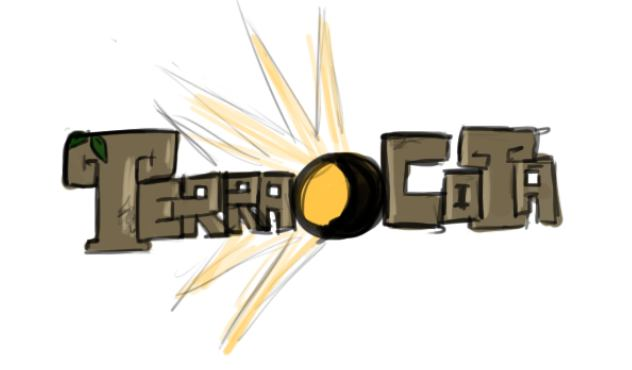
\includegraphics[scale=0.5]{logo-terracota.jpg}
    \caption{Logotipo do jogo Terracota}
    \label{fig:terracota_logo}
\end{figure}

\paragraph{} As logos a seguir representam as tecnologias envolvidas.

\begin{figure}[!htb]
	\centering
	\begin{minipage}{0.5\textwidth}
		\centering
		
\includegraphics[scale=0.1]{logo-vim.png}
		\caption{Editor de Texto Vim}
		\label{Vim logo}
	\end{minipage}%
	\begin{minipage}{0.5\textwidth}
		\centering
		
\includegraphics[scale=0.23]{logo-sublime.png}
		\caption{Editor de Texto Sublime Text}
		\label{Sublime Text logo}
	\end{minipage}
\end{figure}

\begin{figure}[!htb]
	\centering
		\begin{minipage}{0.5\textwidth}
		\centering
		
\includegraphics[scale=0.15]{logo-gnu-linux.png}
		\caption{SO GNU/Linux}
		\label{GNU/Linux logo}
	\end{minipage}%
	\begin{minipage}{0.5\textwidth}
		\centering
		
\includegraphics[scale=0.3]{logo-sdl.png}
		\caption{Biblioteca para desenvolvimento Simple DirectMedia Layer}
		\label{SDL logo}
	\end{minipage}
\end{figure}

\begin{figure}[!htp]
    \centering
    
\includegraphics[scale=0.3]{faixa_etaria.png}
    \caption{Classificação indicativa}
    \label{fig:faixa_indicativa}
\end{figure}

\newpage
\section{Objetos Colecionáveis}
Esta seção contempla a descrição dos objetos colecionáveis do jogo.

\subsection{Primeira Espada}
Encontrada no primeiro nível, recebida do NPC Ferreiro. Possibilita ao jogador
o movimento de ataque.

\begin{figure}[!htb]
    \centering
    
\includegraphics[scale=0.5]{sword1.png}
    \caption{Primeira Espada}
    \label{fig:primeira_espada}
\end{figure}

\subsection{Segunda Espada}
Encontrada na segunda torre, na qual mora Killa. Recebida após encontrar
um baú de tesouro nesta torre. Possibilita ao jogador o movimento de ataque.

\begin{figure}[!htb]
    \centering
    
\includegraphics[scale=0.5]{sword2.png}
    \caption{Segunda Espada}
    \label{fig:segunda_espada}
\end{figure}

\newpage
\section{Telas}
Esta seção contempla a descrição das telas do Terracota.

\subsection{Attract mode}
Para atrair a atenção do jogador, antes de iniciar uma partida, na tela de
abertura, caso tenha decorrido {\bf 10 minutos} sem nenhum input do jogador,
será exibido {\bf concepts arts} do jogo, tais como:

\begin{figure}[hp]
    \centering
    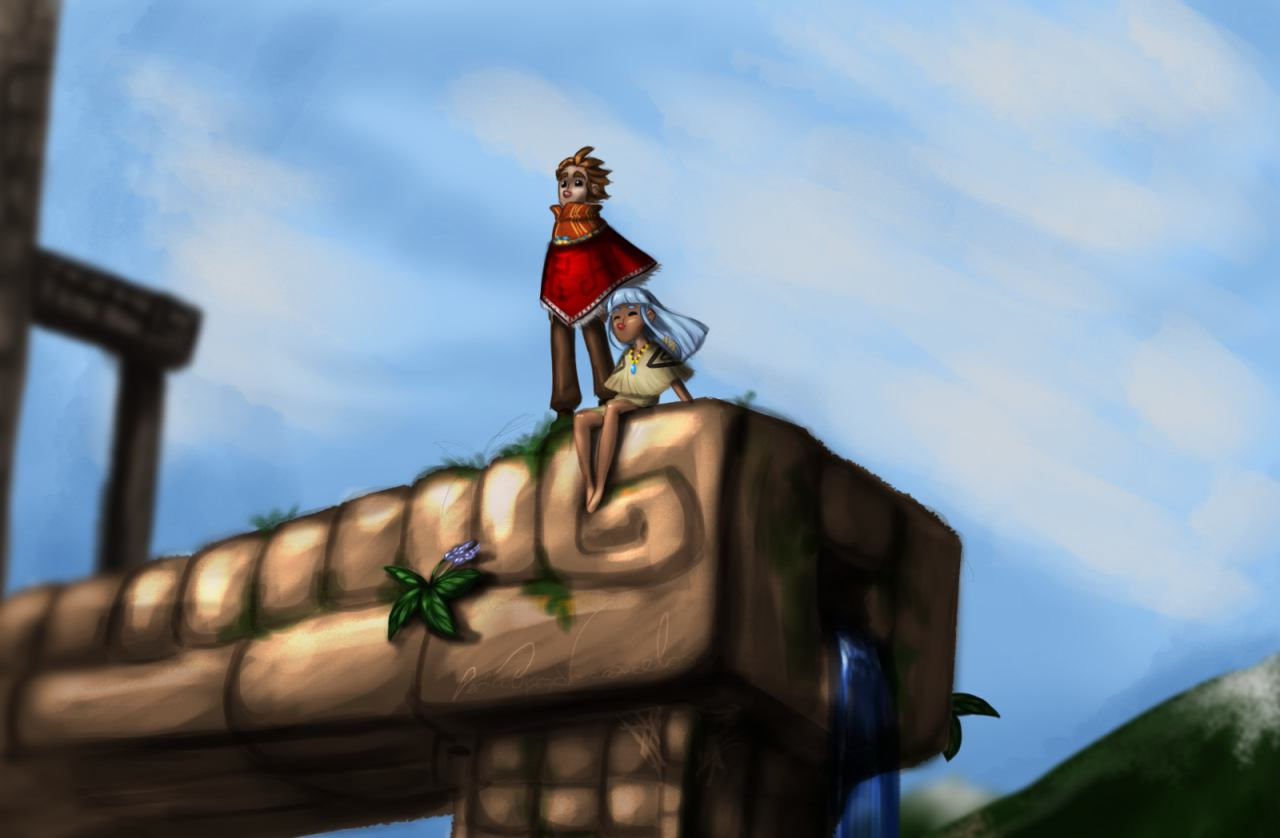
\includegraphics[scale=0.3]{concept_art_01.jpg}
    \caption{Concept Art 01 - Inti e Killa}
    \label{fig:concept_art_01}
\end{figure}

\begin{figure}[hp]
    \centering
    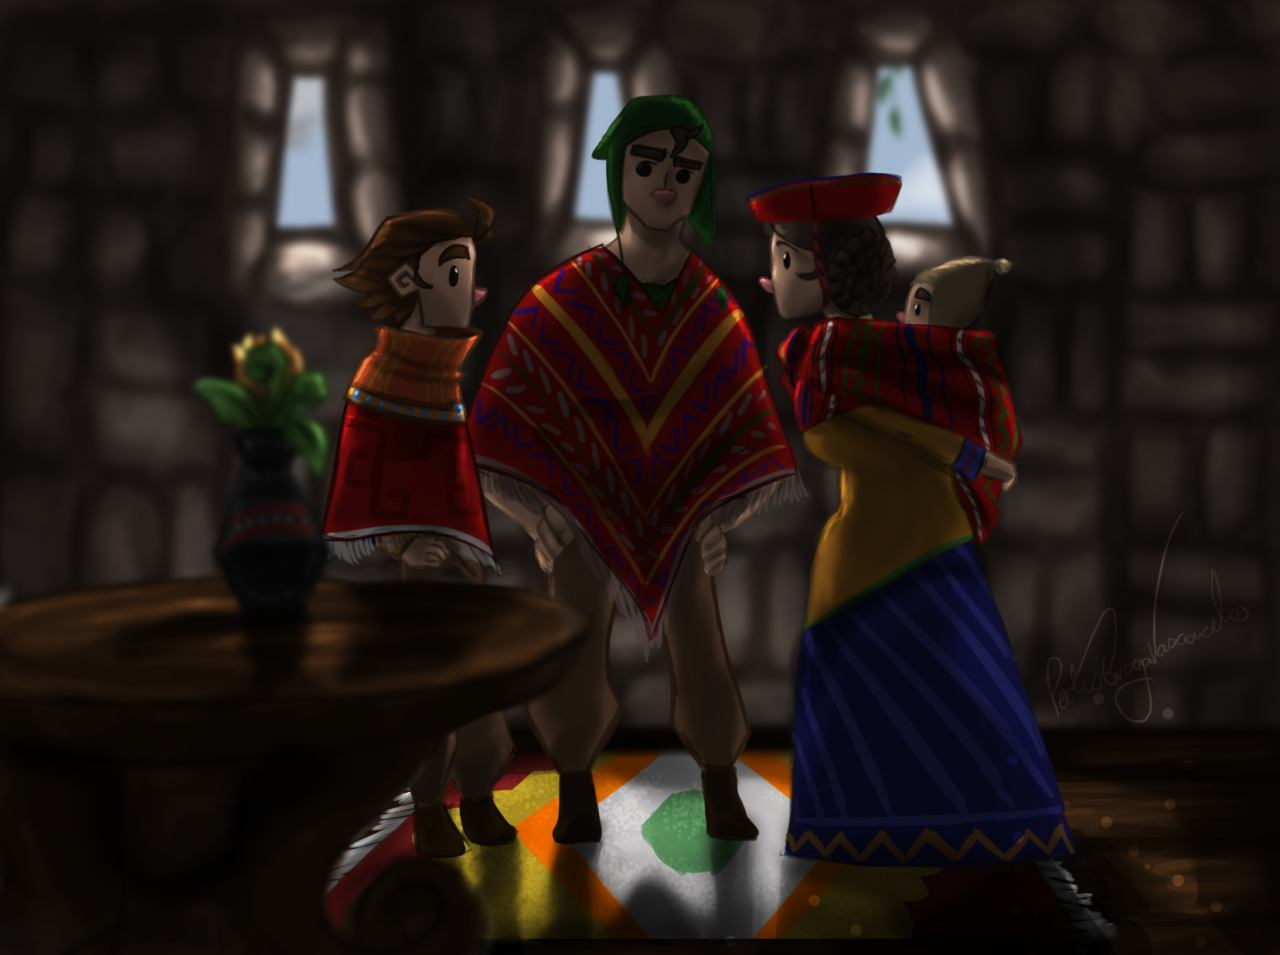
\includegraphics[scale=0.3]{concept_art_02.jpg}
    \caption{Concept Art 02 - Família do Inti}
    \label{fig:concept_art_02}
\end{figure}

\begin{figure}[hp]
    \centering
    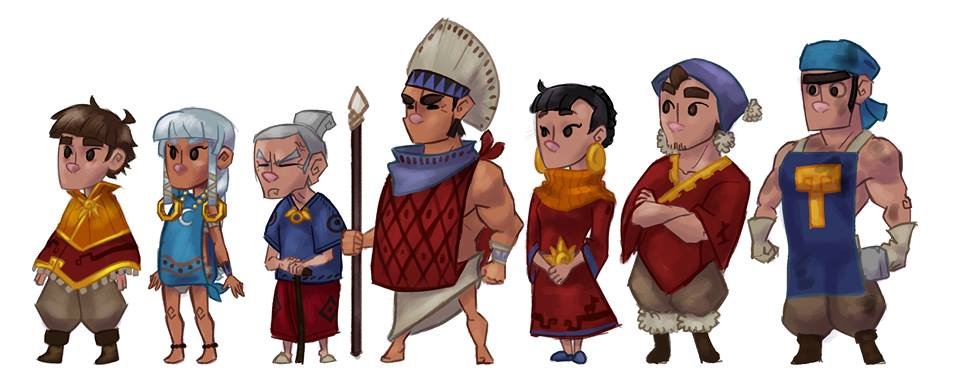
\includegraphics[scale=0.4]{concept_art_03.jpg}
    \caption{Concept Art 03 - Todos os personagens}
    \label{fig:concept_art_03}
\end{figure}

\begin{figure}[hp]
    \centering
    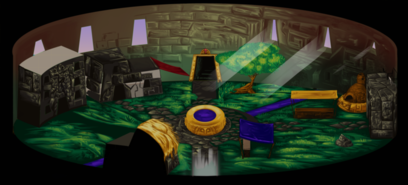
\includegraphics[scale=0.4]{concept_art_04.png}
    \caption{Concept Art 04 - Cenário 01 - Torre 1 - Andar do mercado}
    \label{fig:concept_art_04}
\end{figure}

\begin{figure}[hp]
    \centering
    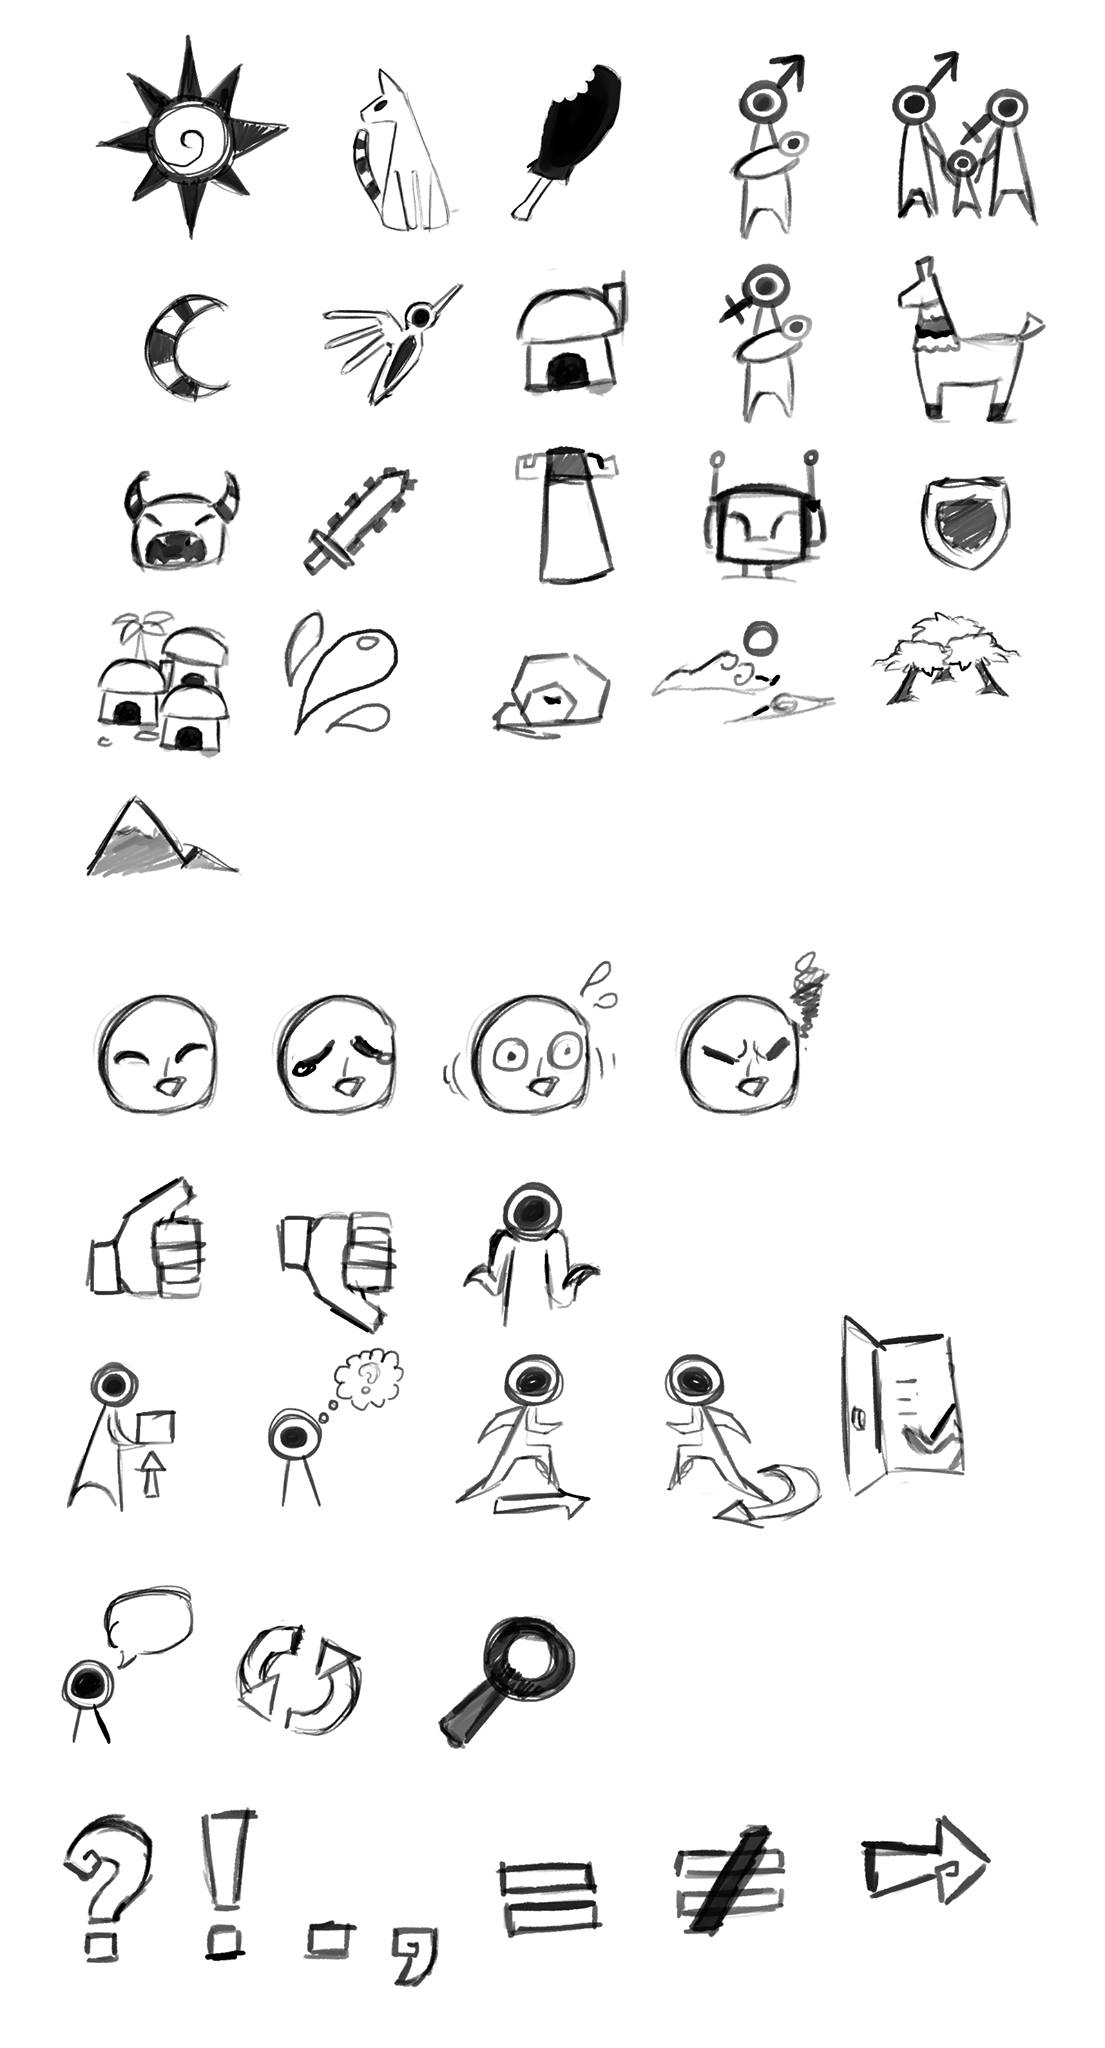
\includegraphics[scale=0.16]{concept_art_05.jpg}
    \caption{Concept Art 05 - Símbolos}
    \label{fig:concept_art_05}
\end{figure}

\newpage
\subsection{Tela de Abertura}
A tela de abertura do jogo Terracota compreenderá dois estados: o de início e
continuação do jogo; e o estado das opções. Será utilizado uma imagem com a
logo do jogo e para cada opção um símbolo correspondente à opção. Por exemplo,
para o botão de início do jogo, será utilizado uma seta para direita, símbolo
convencionado como de "Play". Estas imagens do fundo e dos botões ainda não
estão elaboradas. Como alternativa, apenas para o desenvolvimento e provisoriamente,
serão utilizadas as seguintes imagens.

As opções de início serão (não necessariamente nesta ordem):

\begin{itemize}
    \item Start
    \item Options
    \item Quit
    \item Continue
\end{itemize}


\begin{figure}[!htb]
	\centering
	\begin{minipage}{0.5\textwidth}
		\centering
		
\includegraphics[scale=1]{menu_buttom/start_idle.png}
		\caption{Start Idle}
		\label{start_idle}
	\end{minipage}%
	\begin{minipage}{0.5\textwidth}
		\centering
		
\includegraphics[scale=1]{menu_buttom/start_active.png}
		\caption{Start Active}
		\label{start_active}
	\end{minipage}
\end{figure}

\begin{figure}[!htb]
	\centering
	\begin{minipage}{0.5\textwidth}
		\centering
		
\includegraphics[scale=1]{menu_buttom/options_idle.png}
		\caption{Options Idle}
		\label{options_idle}
	\end{minipage}%
	\begin{minipage}{0.5\textwidth}
		\centering
		
\includegraphics[scale=1]{menu_buttom/options_active.png}
		\caption{Options Active}
		\label{options_active}
	\end{minipage}
\end{figure}

\begin{figure}[!htb]
	\centering
	\begin{minipage}{0.5\textwidth}
		\centering
		
\includegraphics[scale=1]{menu_buttom/quit_idle.png}
		\caption{Quit Idle}
		\label{quit_idle}
	\end{minipage}%
	\begin{minipage}{0.5\textwidth}
		\centering
		
\includegraphics[scale=1]{menu_buttom/quit_active.png}
		\caption{Quit Active}
		\label{quit_active}
	\end{minipage}
\end{figure}

\begin{figure}[!htb]
	\centering
	\begin{minipage}{0.5\textwidth}
		\centering
		
\includegraphics[scale=1]{menu_buttom/continue_idle.png}
		\caption{Continue Idle}
		\label{continue_idle}
	\end{minipage}%
	\begin{minipage}{0.5\textwidth}
		\centering
		
\includegraphics[scale=1]{menu_buttom/continue_active.png}
		\caption{Continue Active}
		\label{continue_active}
	\end{minipage}
\end{figure}

\newpage
As opções de configuração/options serão (não necessariamente nesta ordem):

\begin{itemize}
    \item Fullscreen
    \item Window Mode
    \item Back
\end{itemize}

\begin{figure}[!htb]
	\centering
	\begin{minipage}{0.5\textwidth}
		\centering
		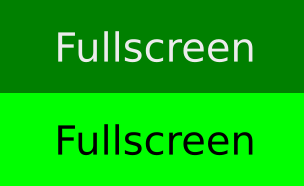
\includegraphics[scale=0.6]{menu_buttom/fullscreen_mode_button.png}
		\caption{Fullscreen Mode}
		\label{fullscreen_mode}
	\end{minipage}%
	\begin{minipage}{0.5\textwidth}
		\centering
		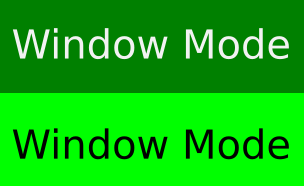
\includegraphics[scale=0.6]{menu_buttom/window_mode_button.png}
		\caption{Window Mode}
		\label{window_mode}
	\end{minipage}
\end{figure}

\begin{figure}[!htb]
    \centering
    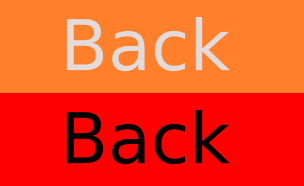
\includegraphics[scale=0.6]{menu_buttom/back_button.png}
    \caption{Back Button}
    \label{fig:back_button}
\end{figure}

\newpage
E a imagem de fundo temporariamente poderá ser esta:

\begin{figure}[!htb]
    \centering
    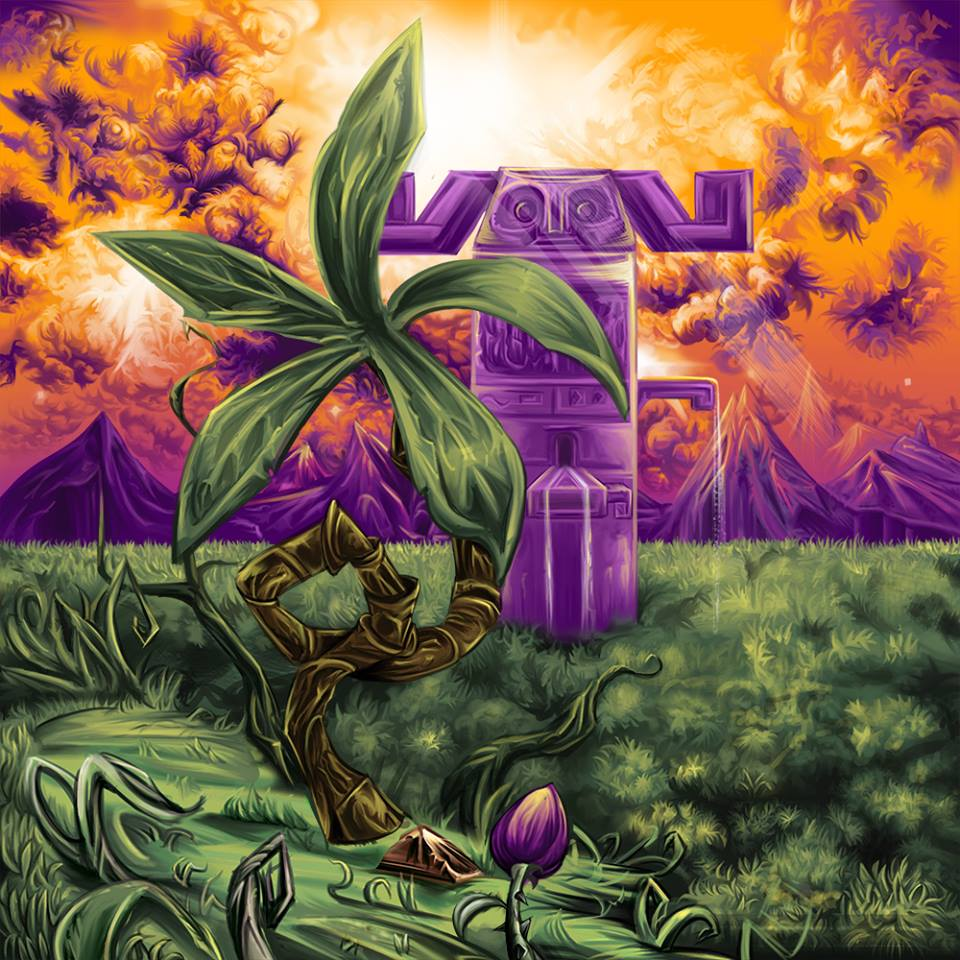
\includegraphics[scale=0.4]{background_terracota.jpg}
    \caption{Tela de Abertura - Backgroud}
    \label{fig:background_terracota}
\end{figure}

\subsection{Outras telas}
Não estarão presentes no Terracota outras telas como créditos e loading screen.

\newpage
\section{Câmera e HUD}

\subsection{Câmera}
A câmera será na "posição" 2.5D. Para melhor visualização deste posicionamento
veja a Figura \ref{fig:camera_hud_01}. O comportamento da camêra será o movimento automático, de
acordo com o posicionamento da personagem principal.

\begin{figure}[!htb]
    \centering
    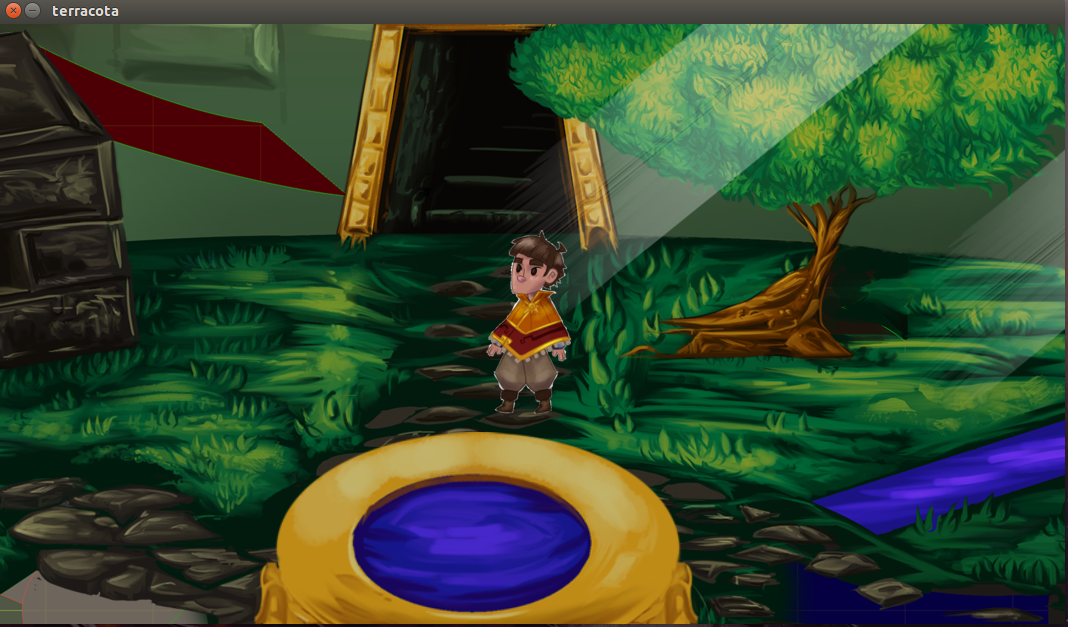
\includegraphics[scale=0.37]{camera_hud_01.png}
    \caption{Demonstração da Câmera}
    \label{fig:camera_hud_01}
\end{figure}

\subsection{HUD}
O HUD (Heads-Up Display) do jogo conterá com uma imagem da barra de vida dos
personagens principais que estarão sendo controlados pelo jogador no momento
quando alternados: ora a barra de vida do Inti, ora da Killa. Os quadrados da
cor verde irão representar a quantidade de vida nesta barra.

Outro elemento exibido no HUB é o botão para alternar entre os personagens.

As imagens a seguir exemplificam como será a HUD:

\newpage

\begin{figure}[!htb]
    \centering
    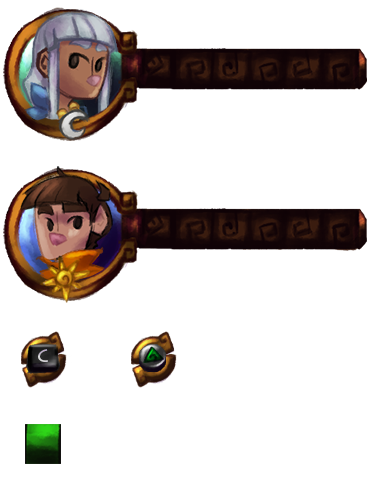
\includegraphics[scale=0.45]{camera_hud_02.png}
    \caption{HUD - Elementos}
    \label{fig:camera_hud_02}
\end{figure}

\begin{figure}[!htb]
    \centering
    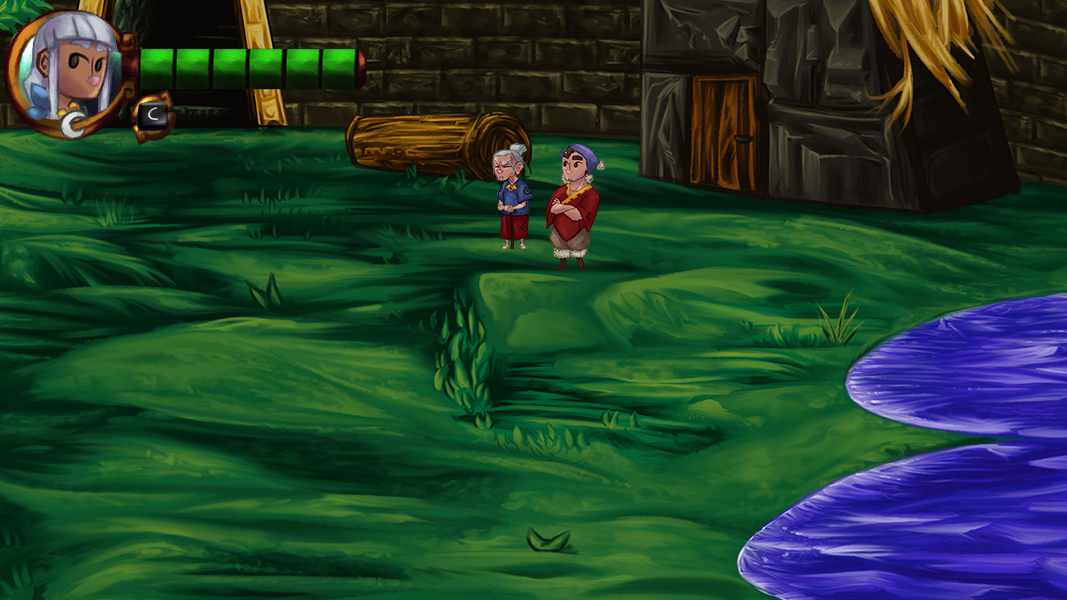
\includegraphics[scale=0.38]{camera_hud_03.png}
    \caption{HUD - Disposição dos Elementos}
    \label{fig:camera_hud_03}
\end{figure}

\newpage

\section{Personagens Principais}
\subsection{Descrição}
\subsubsection{Descrição - Inti}
A escolha do nome Inti é referência ao deus da metologia Inca representado pelo
sol. O garoto Inti Vive na primeira torre do jogo. Seu relacionamento com todos
habitantes desta torre é bastante amigável. Um dia, por algum motivo, ele acaba
encontrando a saída da torre, e ao descobrir que existe algo além da torre,
decide explorar.

A seguir é exibido uma arte conceitual que serviu de inspiração para a identidade
deste personagem e a arte final do mesmo.

\begin{figure}[!htb]
    \centering
    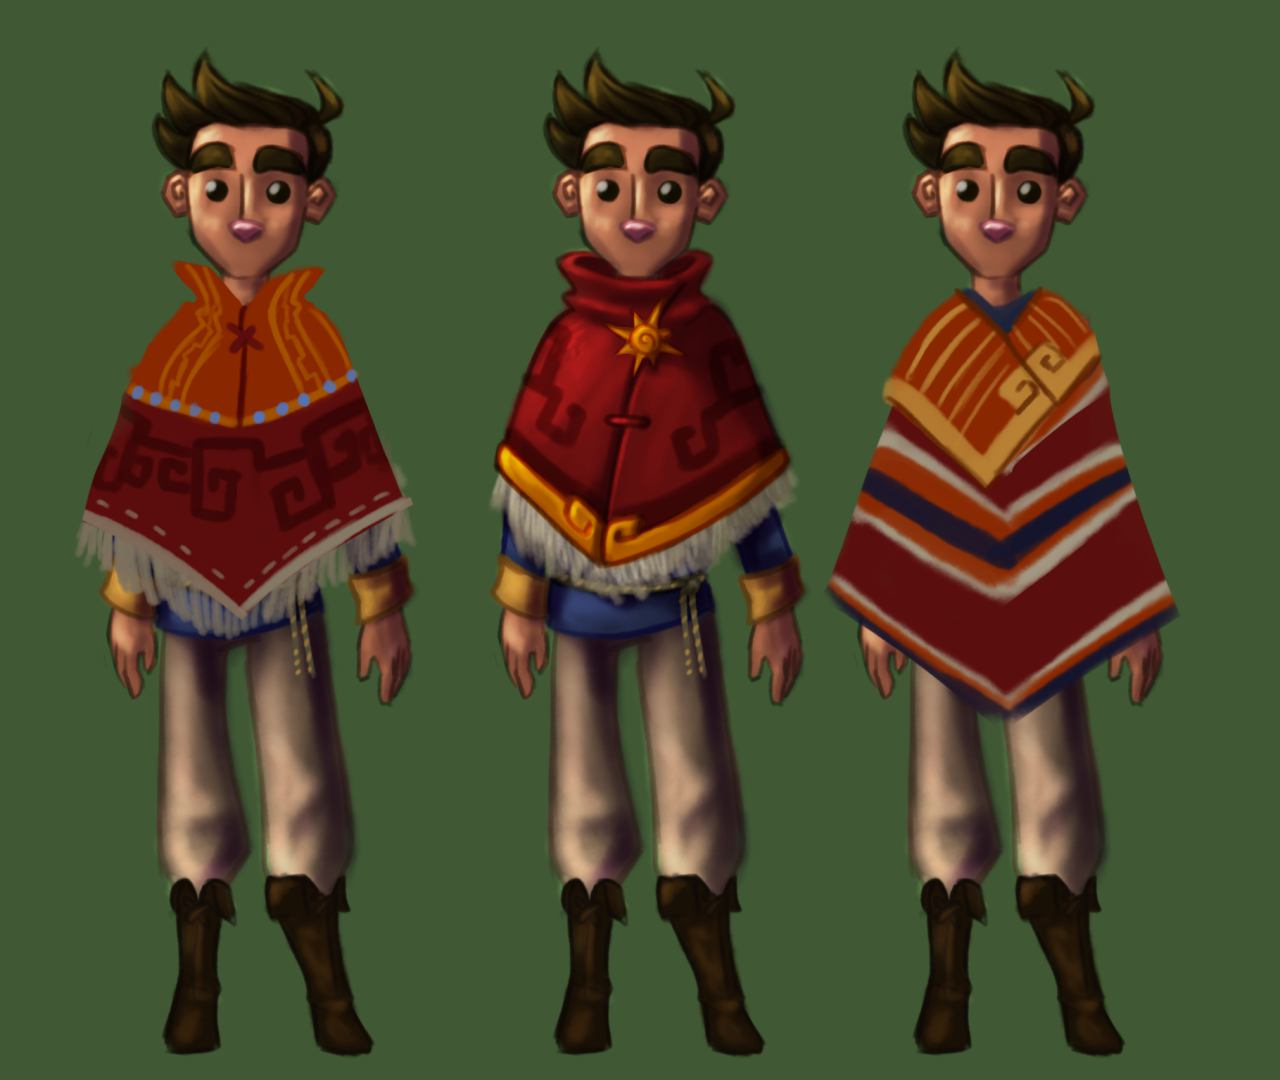
\includegraphics[scale=0.15]{inti_conceitual.jpg}
    \caption{Inti - Arte Conceitual}
    \label{fig:inti_conceitual}
\end{figure}

\begin{figure}[!htb]
    \centering
    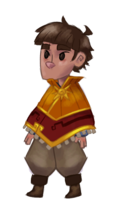
\includegraphics[scale=0.71]{inti_final.png}
    \caption{Inti - Arte Final}
    \label{fig:inti_final}
\end{figure}

\newpage

\subsubsection{Descrição - Killa}
Killa é uma referência à deusa Mama Killa, irmã e esposa do deus Inti da
mitologia, representada pela lua. Aventureira e querida pela tribo. Vive fora de
qualquer torre: na floresta vizinha à torre de Inti. Suas motivações no jogo
iniciam ao interagir com Inti assim que este abandona sua torre natal.

A seguir é exibido uma arte conceitual que serviu de inspiração para a identidade
desta personagem e a arte final do mesmo.

\begin{figure}[!htb]
    \centering
    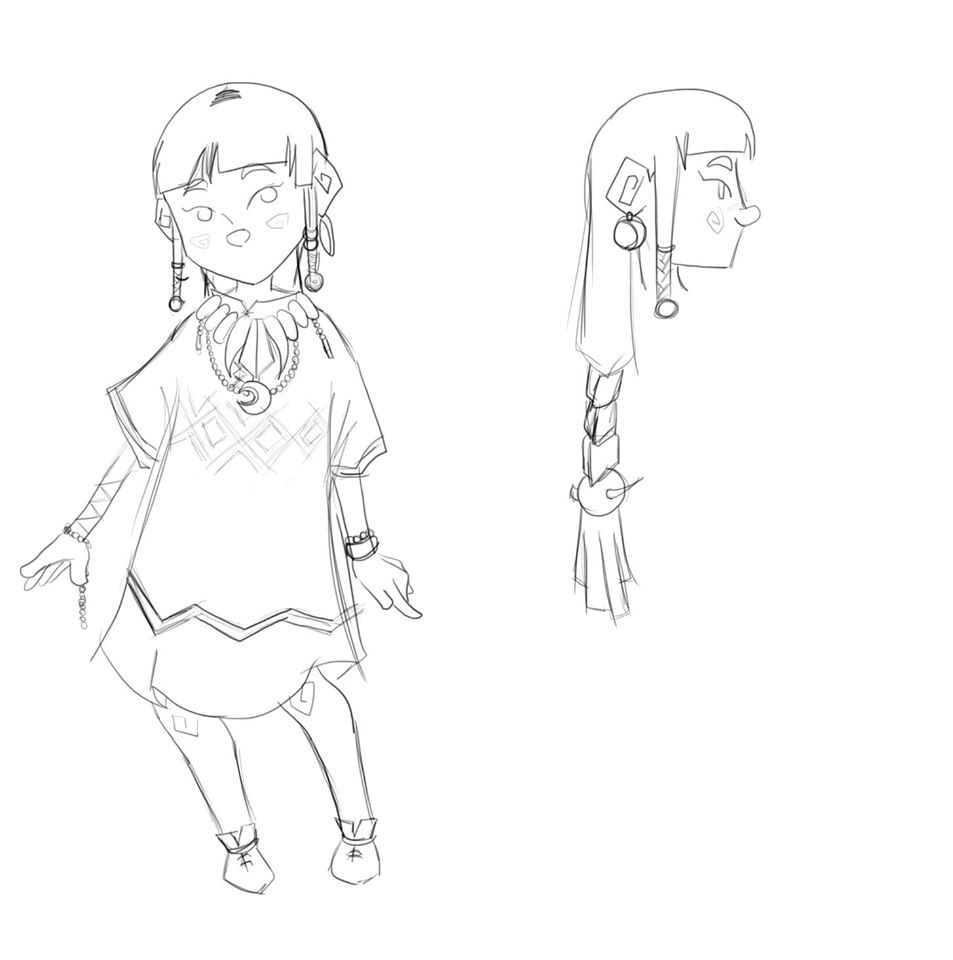
\includegraphics[scale=0.2]{killa_conceitual.jpg}
    \caption{Killa - Arte Conceitual}
    \label{fig:kilaa_conceitual}
\end{figure}

\begin{figure}[!htb]
    \centering
    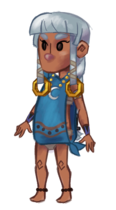
\includegraphics[scale=0.7]{killa_final.png}
    \caption{Killa - Arte Final}
    \label{fig:killa_final}
\end{figure}

\newpage

\subsection{Atributos}
\subsubsection{Inti e Killa}
A proporção do tamanho do Inti e da Killa em relação à tela será XXXXX vezes
menor. A movimentação será na forma de uma caminhada, com a \lq\lq velocidade\rq\rq de 160
pixels/segundos. Outros tipos de navegação (nado, voo, pulo) não estarão
presentes no jogo.

Como movimento sensível ao contexto, haverá o movimento/animação de interação,
que consiste em um simples levantar de mão. Essa interação ocorrerá com os NPCs
e com outros elementos do cenário (por exemplo portas fechadas).

O {\bf dano} causado pelo inimigo Morcego irá retirar um dos 6 espaços de vida de
Inti. E o dano causada por qualquer um dos chefões (Robô ou Camaleão) irá
retirar 2 espaços da barra de vida. A {\bf reação ao dano} será com uma animação
que deixa o personagem transparente por {\bf 3 segundos} e o deixará imune à
qualquer outro dano.

\subsection{Habilidades}
Não haverá habilidades especiais para nenhum dos personagens principais, apenas
um ataque simples descrito na subseção {\bf Combate} a seguir.

\subsection{Inventário}
Os personagens principais não terão o inventário em si. Ambos (Inti e Killa)
possuirão uma ferramenta única de combate: a espada para o Inti e o arco para a
Killa.

\subsection{Combate}
\subsubsection{Combate - Inti}
O ataque do Inti será corpo-a-corpo com uma espada. A movimento será vertical,
de cima pra baixo. A velocidade será aproximadamente XXXXX pixels/segundo. Quando
acionada pela tecla/botão de atacar, irá realizar toda a animação com um único
toque, e caso a tecla continue sendo pressionada a animação  não será repetida,
necessitando assim que o jogador toque várias vezes a tecla/botão para repetidos
ataques. Não haverá uma barra com estamina ou qualquer outro elemento que limite
a quantidade de ataques. Mesmo que o jogo tenha uma temática baseada em jogos
Beat 'em up, o jogador não poderá realizar combos com o ataque. Cada ataque tira
{\bf um espaço} de vida dos inimigos.

A imagem a seguir mostra o Inti em um dos quadros da animação de ataque.

\begin{figure}[!htb]
    \centering
    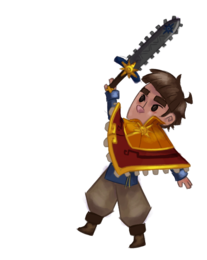
\includegraphics[scale=0.8]{attack_00.png}
    \caption{Inti - Primeiro Quadro da Animação de Ataque}
    \label{fig:inti_attack}
\end{figure}

\subsubsection{Combate - Killa}
O ataque da Killa será à distância utilizando arco e flecha. O alcance da flecha
será fixo, mas ainda não está definido. A velocidade da flecha será aproximadamente
de XXXXX pixels/segundo. Quando acionada a tecla/botão de ataque, a animação será
toda a animação de ataque uma única vez para cada toque, ou seja, uma flecha
lançada por toque. Quando a tecla for pressionada, não será lançado flechas
indiscriminadamente. Não haverá uma barra com estamina ou qualquer outro
elemento que limite a quantidade de ataques. Mesmo que o jogo tenha uma temática
baseada em jogos Beat 'em up, o jogador não poderá realizar combos com o ataque.
Cada ataque tira {\bf um espaço} de vida dos inimigos.

A imagem a seguir mostra a Killa em um dos quadros da animação de ataque.

\begin{figure}[!htb]
    \centering
    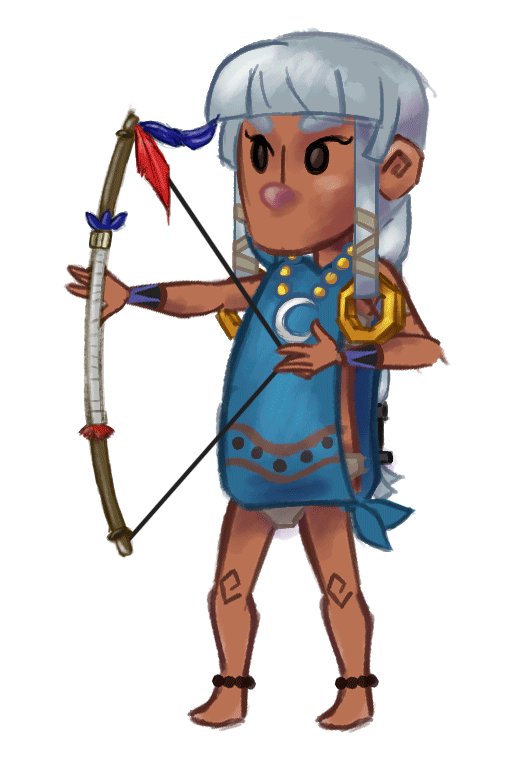
\includegraphics[scale=0.2]{killa_attack.png}
    \label{fig:killa_attack}
    \caption{Killa - Quadro da Animação de Ataque}
\end{figure}

\newpage

\section{Principais Personagens do Mundo do Jogo}

\subsection{Pais do Inti}
Os pais do personagem principal Inti criaram seu filho incentivando o espírito
investigador e colaborativo, pois toda a sociedade da primeira torre necessita
da toda ajuda possível para a sua continuidade. Ambos nasceram já com a primeira
torre construída. Por essa fato, negam para Inti a possibilidade da existência
de uma outra civilização fora da torre logo que este retorna da aldeia onde
conversou com o cacique.

A mãe é amorosa e o pai é forte e demonstra vigor, como é preciso ter em um
mundo pós-apocalíptico. Ambos possuem idade superior aos 40 anos. E o visual
proposto para ambos está na imagem a seguir.

\begin{figure}[!htb]
    \centering
    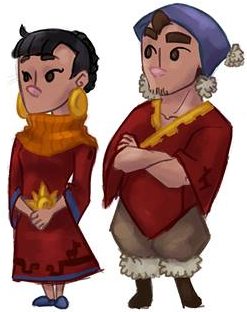
\includegraphics[scale=0.9]{pais_do_inti.jpg}
    \label{fig:pais_do_inti}
    \caption{Pais do Inti}
\end{figure}

\newpage

\subsection{Cacique}
Embora sua aparência seja de alguém jovem, o Cacique é um homem bastante
experiente. Ele é quem conta toda a história de reconstrução da sociedade
humana para Inti. Conhecido por conversar por longos períodos de tempo, educa
sua filha, Killa (a outra personagem principal), de uma forma livre, mas sempre
supervisionada e aconselhada. Passa todos os conhecimentos sobre os desafios que
Killa talvez possa encontrar nas florestas. E é ele quem ensina também Killa a
utilizar o arco e a flecha.

Sua idade não é bem estabelecida, porém aparenta ter quase a mesma idade que os
pais de Inti. E por seu elevado cargo/papel na aldeia, seu porte físico é
superior ao do pai de Inti e até mesmo do Ferreiro da Primeira Torre. O visual
do Cacique é o proposto na imagem a seguir.

\begin{figure}[!htb]
    \centering
    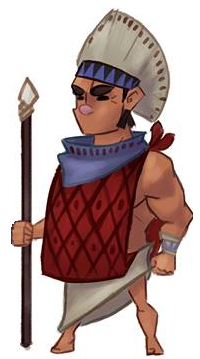
\includegraphics[scale=0.9]{cacique_pai_da_killa.jpg}
    \label{fig:cacique_pai_da_killa}
    \caption{Cacique e Pai da Killa}
\end{figure}

\newpage

\section{Progresso do Jogo}

\subsection{Cenário 1 - Torre 1 - Andar do Mercado}
O primeiro cenário jogável encontra-se na Torre 1, e possui o nome de (apenas
para controle interno) Andar do Mercado. O objetivo principal do jogador no
nível é:

\begin{itemize}
    \item Conversar com a Mãe do Inti - Missão de levar comida para o Pai;
    \item Conversar com a Sogra - Missão dos Morcegos;
    \item Conversar com o Ferreiro para receber a Primeira Espada.
\end{itemize}

Neste nível está localizada a casa de Inti e a de outros habitantes da Primeira
Torre. Além de outros elementos, como a barraca do Ferreiro e uma barraca para
referenciar um mercado. A característica principal desse nível/cenário é a de uma
fonte ou poço no centro. Não haverá inimigos neste nível. É neste nível que é
obtido o primeiro Objeto Colecionável: a Primeira Espada. O tempo estará sempre
claro, de dia. As cores predominantes serão o verde e o marrom das paredes da torre
e das casas. A imagem a seguir mostra este primeiro cenário.

\begin{figure}[!htb]
	\centering
	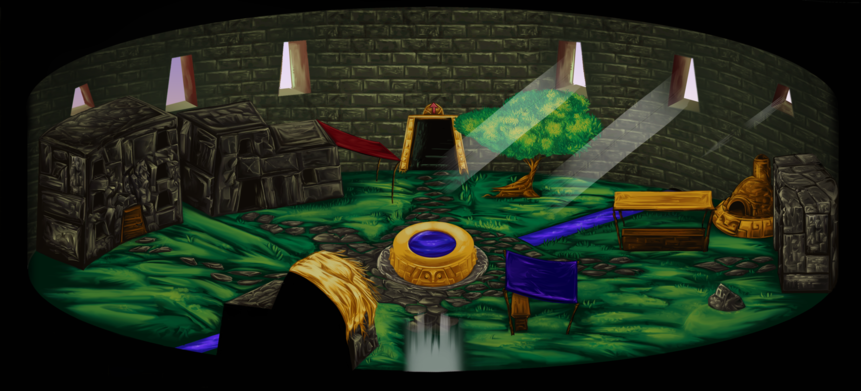
\includegraphics[scale=0.45]{cenario_01.png}
	\label{fig:cenario_01}
	\caption{Cenário 1 - Torre 1 - Andar do Mercado}
\end{figure}

\newpage

\subsection{Cenário 2 - Torre 1 - Andar das Lhamas}
O segundo cenário jogável encontra-se na Torre 1, e possui o nome de (apenas
para controle interno) Andar das Lhamas. O objetivo principal do jogador no
nível é:

\begin{itemize}
    \item Conversar com o Pai do Inti - Completar Missão de levar comida para o
    Pai;
\end{itemize}

Neste nível está localizado pasto das Lhamas, um celeiro e uma pequena moradia.
A característica principal desse nível/cenário é a presença de várias Lhamas.
O Pai do Inti também está neste cenário e o jogador deve entregar a comida para
completar a primeira missão. Não haverá inimigos neste nível, nem objetos
colecionáveis. O tempo estará sempre claro, de dia. As cores predominantes serão
as mesmas do Cenário 1, além das cores diversas das Lhamas. As imagens a seguir
mostram este segundo cenário e as Lhamas.

\begin{figure}[!htb]
	\centering
    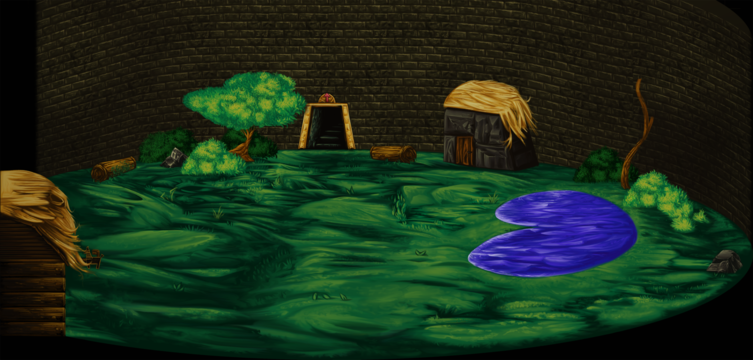
\includegraphics[scale=0.4]{cenario_02.png}
    \label{fig:cenario_02}
    \caption{Cenário 2 - Torre 1 - Andar das Lhamas}
\end{figure}

\begin{figure}[!htb]
	\centering
    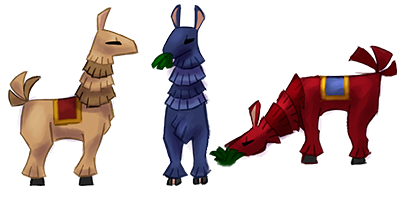
\includegraphics[scale=0.4]{lhamas.png}
    \label{fig:lhamas}
    \caption{Lhamas do Cenário 4}
\end{figure}

\newpage

\subsection{Cenário 4 - Torre 1 - Andar do Boss}

O terceiro cenário jogável encontra-se na Torre 1, e possui o nome de (apenas
para controle interno) Casa do Inti. O objetivo principal do jogador no
nível é:

\begin{itemize}
    \item (sem objetivo específico - somente para visitar)
\end{itemize}

Neste nível está localizado apenas elementos da casa do Inti, como uma mesa,
um balcão e um armário. Não haverá NPCs. Não haverá inimigos neste nível, nem
objetos colecionáveis. Como a Casa é fechada, não é possível saber sobre o tempo
As cores predominantes são marrom e cinza. A imagem a seguir mostra este
terceiro cenário.

\begin{figure}[!htb]
	\centering
    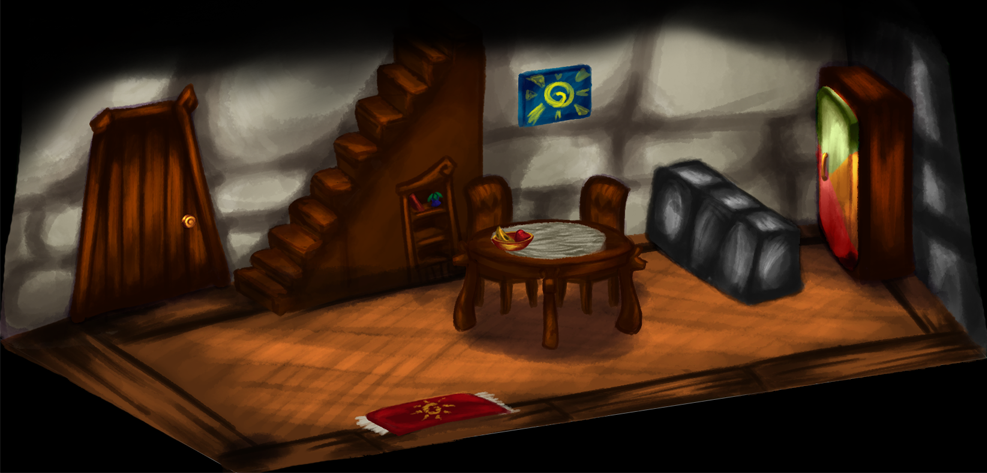
\includegraphics[scale=0.35]{cenario_03.png}
    \label{fig:cenario_03}
    \caption{Cenário 3 - Torre 1 - Casa do Inti}
\end{figure}

\newpage

\subsection{Cenário 4 - Torre 1 - Andar do Boss}

O quarto cenário jogável encontra-se na Torre 1, e possui o nome de (apenas
para controle interno) Casa do Inti. O objetivo principal do jogador no
nível é:

\begin{itemize}
    \item Derrotar todos os Morcegos - Missão entregue pela Sogra
    \item Derrotar o boss Robô - Necessário para sair da Torre 1
\end{itemize}

Neste nível estão localizados os dois inimigos do jogo: o Morcego e o Robô.
Conterá um círculo no centro, remendos de metal nas paredes e um portal de saída
da Torre 1. Não haverá NPCs neste cenário. Para cumprir os objetivos, o jogador
terá que derrotar os dois inimigos. Não haverá objetos colecionáveis. O tempo
estará sempre claro, de dia. As cores predominantes serão marrom e o amarelo
do portal. A imagem a seguir mostra este quarto cenário.

\begin{figure}[!htb]
	\centering
    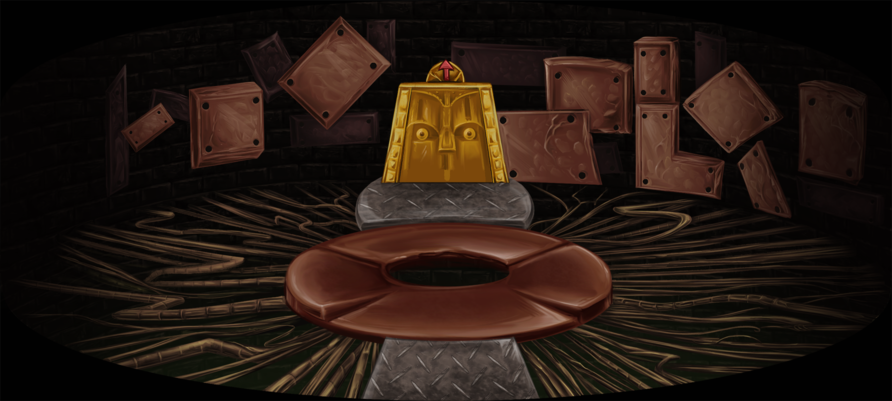
\includegraphics[scale=0.4]{cenario_04.png}
    \label{fig:cenario_04}
    \caption{Cenário 4 - Torre 1 - Andar do Boss}
\end{figure}

\end{document}
